\graphicspath{{./main/2_introduction/figures/}}

\chapter{Introduction}
\label{chap:intro}

\vspace{-10mm}
\section{Ground Autonomous Vehicles}
\begin{figure}[H]
	\centering
	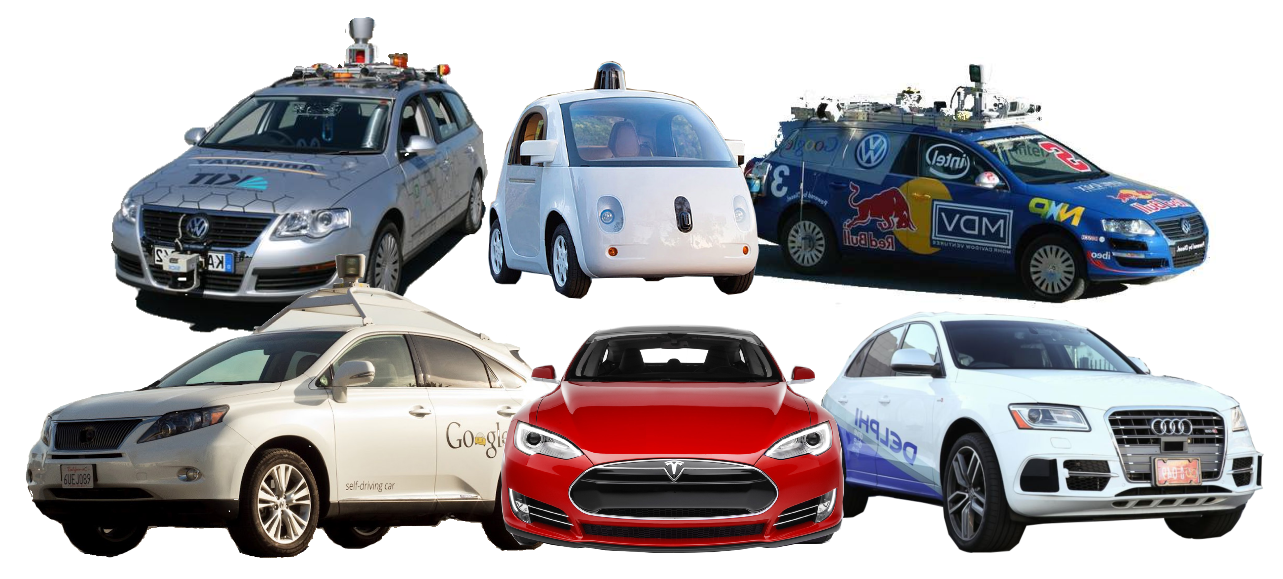
\includegraphics[width=1\textwidth]{driverless2.eps}
	\caption{Examples of Ground Autonomous Vehicles.}
	\label{fig:00_driverless}
\end{figure}

Autonomous Vehicles (AVs) and more specifically their ground counterpart, Ground Autonomous Vehicles (GAVs), have become one of the most revolutionary technologies of the beginning of this century. These vehicles are expected to cause a large social impact in the near future, providing us with a reliable and affordable source of transportation, reducing road fatalities, causing a more steady flow of traffic, reducing fuel consumption and noxious emissions, as well as improving driver comfort and enhance mobility for elderly and handicapped persons~\cite{Woensel:2015}. GAVs can be seen as the natural evolution of Advanced Driver Assistance Systems (ADAS), which aim to improve traffic safety by assisting drivers via warnings and performing controlled counteractive measures in dangerous situations. 

The principal representative of GAVs is the autonomous car, which is the name that robotics cars receive. Autonomous cars and GAVs in general are  robotic platforms endowed with a set of sensors to perceive their environment (\eg cameras, radars, lasers, etc.), actuators to interact with the environment (\eg automatic steering, acceleration, brake, etc.) and processing hardware to run the algorithms required to understand the environment and make decision throughout these sensors and actuators. The combination of all these systems endows GAVs with certain degree of autonomy to navigate. Such levels of autonomy along with the capacities and limitations of autonomous cars have been defined by different organizations. The National Highway Traffic Safety Administration (NHTSA) proposes the following formal classification \cite{wiki:AutonomousCar}:

\begin{itemize}
\item Level 0: The vehicle is totally controlled by a human driver
\item Level 1: Some basic controls are automated \eg braking
\item Level 2: Several controls are automated and can be used together to create an ADAS system, \eg parking assistance 
\item Level 3: The car can operate autonomously controlling all safety-critical functions in certain conditions (\eg highway scenarios), but the driver must supervise the driving and retake control when the vehicle requests it. The vehicle must provide a sufficiently comfortable ''reconnection time'' for the driver.
\item Level 4: The vehicle is fully autonomous, performing all safety-critical functions $100\%$ of the time. The driver is not expected to retake control of the vehicle at any time.
\end{itemize}

An alternative taxonomy has been published by the  Society of Automotive Engineers (SAE):

\begin{itemize}
\item Level 0: Vehicle with no automated control, but capable of issuing warnings
\item Level 1: Vehicle endowed with several automated controls to create ADAS systems, Adaptive Cruise Control (ACC), Parking Assistance with automated steering, and Lane Keeping Assistance (LKA). Driver must be ready to take control at any time
\item Level 2: Driver is on charge of detecting objects and other hazards, responding accordingly when the automated system fails to respond. The automated system executes accelerating, braking, and steering. The automated system can deactivate immediately upon takeover by the driver.
\item Level 3: The vehicle can operate with full autonomy and no human intervention within specific environments, \eg highway
\item Level 4: The vehicle can operate in full autonomy in all but few conditions, such as severe weather. The driver is responsible to activate the system only when it is safe to do so (his/her attention then would not be required)
\item Level 5: Driver sets the destination and starts the system, the vehicle is fully autonomous and requires no intervention
\end{itemize}

The automotive industry has progressively started moving from level 0 to higher levels of autonomy, fuelled by the strong motivation of eliminating ---or at least palliating--- some of the most challenging problems of our era, aiming for:

\begin{itemize}
\item Reducing accidents and fatalities (ideally to 0)
\item Decreasing congestion in urban areas
\item Improving efficiency in road usage
\item Increasing human efficiency 
\item Improving energetic needs for global transportation
\end{itemize}

The plan is to progressively improve on these points on our way to mature NHTSA-level-4 and SAE-level-5 systems. However, developing GAVs with the aforementioned capabilities presents several technological challenges that are yet to be solved. For vehicles to acquire this level of autonomy it is required a very sophisticated comprehension of the surrounding scene; in other words, through its sensors and software a level-4 GAV must be able to process and understand which are the current entities present in the scene, \ie cars, pedestrians, how many of them, etc.; its own situation within the scene, \eg, type of lane in which the vehicle is located; and its situation with respect to other entities of the scene, considering factors such as speed, trajectory and intentions. The process to comprehend all these critical factors is commonly referred to as scene understanding. By definition, scene understanding refers to the task (or set of tasks) enabling an agent to gain a full interpretation of a scene through video, still images or other media, leading to a human-like interpretation and inference of general principles, rules, behaviours and arbitrary situations. In other words, scene understanding is the fundamental capacity of creating a helpful interpretation of our environment; a mental model that represents the first step towards smart decision making. This problem definition is so broad that in practice scene understanding can be seen as a field containing several problems instead of as an atomic entity; and this field largely intersects with the field of computer vision.

The knowledge of a scene is hierarchical, \ie, a scene can be described at different levels of abstraction: it can be described according to the geometry of the scene (\eg, a flat region with a whole in the middle), to respect to the objects it contains (\eg pedestrians, buildings, etc.), according to how these objects are placed on the scene (\eg streets, indoor environment, etc.), in terms of the type of scene, in terms to the actions performed by the objects/entities of the scene (\eg a traffic jam, a fight, etc.), among many other levels~\cite{SceneUnderstanding}. These levels bring different information about a scene and can be addressed as different problems, \eg, localization, object detection, place recognition, semantic segmentation, activity recognition, etc. In this way, the scene understanding task, which is usually considered as a long-term goal, can be decomposed in sub-tasks that simplify and bound its scope.

The different levels of abstraction in scene understanding and the different sub-tasks that they spawn can be viewed according to their level of complexity. In this way, finding our own position on a scene would be at the bottom of the tasks to solve in order to fully understand the scene, followed by the knowledge on how to ``parse'' the elements of the scene considering their associated context (\ie, image parsing or semantic segmentation), and then giving an interpretation of what kind of scene is that (place recognition) and how are their elements interacting (activity recognition). It is therefore, logical to establish a level of maturity for the task of scene understanding according to the degree of maturity obtained when addressing the different levels of abstraction. In this thesis we study how to address these first level of scene understanding, dealing with (ego) localization of a vehicle---\ie, where is the vehicle in the scene?---and semantic segmentation---\ie, what are the objects around me?.

In order to perform these tasks it has proven to be critical to use the right type of sensors. In this way, within the context of driving scenes, visual inputs coming from cameras have become the core source of information to reason about the current situation of traffic, vehicles and other agents. Cameras are a low-cost alternative to active sensors like Lidars and have proven to work well for several scene understanding sub-tasks, as for instance pedestrian detection and obstacle avoidance, reason why they are currently incorporated in all modern vehicles. Thus, since cameras are already there, why not use them to their fullest? The versatility and potentials of cameras in the context of autonomous vehicles is also one of the main motivations of this thesis on visual scene understanding.

\section{Visual Scene Understanding}

Recently, the visual scene understanding ecosystem has lived an important boost due mainly to the triumph of deep learning on several key problems, such as object recognition and semantic segmentation~\cite{LongICCV15Fully}. New approaches based on deep neural networks have proven to achieve a previously never seen level of accuracy and generalization, going beyond human capabilities in some cases~\cite{HeICCV15Delving}. It is believed that all the knowledge that we have acquired on the creation of new models, datasets and hardware will contribute to the realization of visual scene understanding. However, the blooming of deep learning technologies will take years to be considered in a mature enough state so it can be fully deployed in GAVs.

To compensate for the lack of maturity of visual scene understanding, autonomous driving technology has focused on a technological surrogate that helps to simplify the problem: strong priors in the form of fully-annotated high-definition maps. Instead of trying to understand the current scene from scratch, GAVs rely on highly detailed maps of an area, that usually include 3D data, and the semantics associated to the static scene, among others. In this way, ``understanding'' becomes a retrieval process of pre-acquired and pre-annotated information when the precise localization of the vehicle with respect to one of these maps is known. In this way, critical information, as for instance, the limits of navigable regions, driving speeds and dangerous areas can be obtained through a manual or a semi-supervised process offline, which drastically simplifies the cognitive requirements of GAVs. Given this pre-baked knowledge, GAVs can focus on identifying new dynamic events, such as obstacles, pedestrians, other vehicles, the state of traffic lights, etc. These tasks are then carried out by a simplified visual scene understanding module.

In practice, mapping technology is considered mature enough to serve as a solid starting point for developing GAV systems, what motivates that a big part of the automotive industry is designing autonomous cars around this concept. On the other hand, those systems dealing with more abstract levels of understanding are still in an embryonary state, just covering partial functionalities such as pedestrian detection and traffic sign recognition. However, the interest in this type of systems is increasing, since they are considered the next leading technology in the development of GAVs. Currently, these technologies are seen as complementary, but in the future when this part of scene understanding becomes mature enough, both system would be able to operate independently, offering a rich source of redundancy when combined.     

In this thesis we show several contributions to improve important aspects of two scene understanding sub-tasks, namely, visual localization, and semantic parsing of the scene. To this end, this document has been divided in two parts: part I covers the contributions we have done in visual localization, which resides on the side of the spectrum of those methods that are map-dependent. Part II covers our contributions in scene semantic parsing, with techniques that are map independent.


% ----------------------------------------------------------------
\section{Objectives and Scope} 

The aim of this PhD dissertation is to develop new approaches to understand driving scenes by using computer vision, applied mathematics and machine learning. To this end we set the focus of this thesis on visual scene understanding for driving scenarios, proposing new solutions to understand (part I) ``where'' is our autonomous vehicle in the scene and (part II) ``what'' are the objects that surround our vehicle.

With this structure in mind, first we focus on addressing the ``where'', focusing on the task of robust visual localization. To this end, we study and extend geometric methods to produce faster and more reliable localization approaches to operate in real environments. We ask the following questions:

\begin{itemize}
\item Is it possible to exploit compressed regression to create more efficient localization methods?
\item How can we embed robustness into compressed regression techniques?
\item Can we improve localization robustness using robust manifold optimization?
\item Is it possible to exploit rank constraints and sparsity to boost localization accuracy? 
\end{itemize}

The second part of this thesis deals with  the ``what'', focusing on semantic segmentation of the scene and semantic change recognition. Here we propose to use learning-based method and show how these can be combined with maps to improve the computational efficiency of the resulting system. In this part we deal with the following questions:

\begin{itemize}
\item How to exploit maps to embed semantic knowledge and reduce computational time?
\item How to adapt pre-trained scene understanding models to operate in new unseen conditions?
\item How to exploit virtual environments and domain adaptation to improve generalization and accuracy of scene understanding related problems?
\item Can we create new training methods to deal with data multi-modality in deep learning models?
\item How to compress a state-of-the-art model into an embedded device?
\item Can deep learning and virtual worlds solve the problem of change detection in driving scenarios?
\end{itemize}

Bringing light to these questions from the point of view of computer vision and machine learning are the objectives of this PhD. Our aim is to contribute to the understanding and development GAVs and to produce mature systems that can understand their surroundings and make decisions accordingly.

% ----------------------------------------------------------------
\section{Outline}

This PhD thesis has been divided into three parts. The first part of this document, \textit{Where am I on the Scene?}, deals with aspects of visual localization, with special emphasis in localization robustness and efficiency. This part starts with an introduction and motivation to the problem of visual localization in chapter~\ref{chap:p1_00}. In chapter~\ref{chap:p1_01} we deal with embedding techniques and compressed regression to improve efficiency of ego-pose estimation for visual localization. These ideas are extended in chapter~\ref{chap:p1_02} where we study how to use data embeddings and robust manifold optimization to increase robustness for pose estimation in localization problems. Chapter~\ref{chap:p1_03} studies an alternative viewpoint to localization and pose estimation, making use of the inner low-rank and sparsity constraints of the problem to propose a Robust PCA approach. The methods proposed in chapter~\ref{chap:p1_03} are further improved in chapter~\ref{chap:p1_04} into an efficient Robust PCA method to deal with larger data volumes. 

The second part of this document, \textit{What is on the Scene?}, deals with aspects of semantic segmentation and change detection, with special emphasis to practical problems, such as compressing models to operate in embedded devices and adapting models to work in new conditions using transfer learning and domain adaptation. First, chapter~\ref{chap:p2_00} provides a general  introduction to these problems. Then in chapter~\ref{chap:p2_01} we propose a new strategy  based on the combination of mapping, localization and information retrieval to develop a real-time scene understanding approach. Chapter~\ref{chap:p2_02} deals with the problem of deploying semantic segmentation models in new unseen scenarios using online unsupervised adaptation. In chapter~\ref{chap:p2_03} we cover practical methods to train semantic segmentation models for driving environments, showing how to address data multi-modality issues and model compression for its use in embedded devices. Chapter~\ref{chap:p2_04} describes how the combination of virtual environments and domain adaptation can dramatically improve semantic segmentation approaches based on deep-learning. In chapter~\ref{chap:p2_05} we show that change detection and semantic change detection can be addressed as variations of semantic segmentation and how to make this possible by exploiting virtual worlds. Finally, in part III, \textit{Clausula}, within chapter~\ref{chap:end}, we presents the conclusion of this PhD thesis along with a summary of scientific contributions, patents and related deliverables of this thesis.